
% Default to the notebook output style

    


% Inherit from the specified cell style.




    
\documentclass[11pt]{article}

    
    
    \usepackage[T1]{fontenc}
    % Nicer default font (+ math font) than Computer Modern for most use cases
    \usepackage{mathpazo}

    % Basic figure setup, for now with no caption control since it's done
    % automatically by Pandoc (which extracts ![](path) syntax from Markdown).
    \usepackage{graphicx}
    % We will generate all images so they have a width \maxwidth. This means
    % that they will get their normal width if they fit onto the page, but
    % are scaled down if they would overflow the margins.
    \makeatletter
    \def\maxwidth{\ifdim\Gin@nat@width>\linewidth\linewidth
    \else\Gin@nat@width\fi}
    \makeatother
    \let\Oldincludegraphics\includegraphics
    % Set max figure width to be 80% of text width, for now hardcoded.
    \renewcommand{\includegraphics}[1]{\Oldincludegraphics[width=.8\maxwidth]{#1}}
    % Ensure that by default, figures have no caption (until we provide a
    % proper Figure object with a Caption API and a way to capture that
    % in the conversion process - todo).
    \usepackage{caption}
    \DeclareCaptionLabelFormat{nolabel}{}
    \captionsetup{labelformat=nolabel}

    \usepackage{adjustbox} % Used to constrain images to a maximum size 
    \usepackage{xcolor} % Allow colors to be defined
    \usepackage{enumerate} % Needed for markdown enumerations to work
    \usepackage{geometry} % Used to adjust the document margins
    \usepackage{amsmath} % Equations
    \usepackage{amssymb} % Equations
    \usepackage{textcomp} % defines textquotesingle
    % Hack from http://tex.stackexchange.com/a/47451/13684:
    \AtBeginDocument{%
        \def\PYZsq{\textquotesingle}% Upright quotes in Pygmentized code
    }
    \usepackage{upquote} % Upright quotes for verbatim code
    \usepackage{eurosym} % defines \euro
    \usepackage[mathletters]{ucs} % Extended unicode (utf-8) support
    \usepackage[utf8x]{inputenc} % Allow utf-8 characters in the tex document
    \usepackage{fancyvrb} % verbatim replacement that allows latex
    \usepackage{grffile} % extends the file name processing of package graphics 
                         % to support a larger range 
    % The hyperref package gives us a pdf with properly built
    % internal navigation ('pdf bookmarks' for the table of contents,
    % internal cross-reference links, web links for URLs, etc.)
    \usepackage{hyperref}
    \usepackage{longtable} % longtable support required by pandoc >1.10
    \usepackage{booktabs}  % table support for pandoc > 1.12.2
    \usepackage[inline]{enumitem} % IRkernel/repr support (it uses the enumerate* environment)
    \usepackage[normalem]{ulem} % ulem is needed to support strikethroughs (\sout)
                                % normalem makes italics be italics, not underlines
    

    
    
    % Colors for the hyperref package
    \definecolor{urlcolor}{rgb}{0,.145,.698}
    \definecolor{linkcolor}{rgb}{.71,0.21,0.01}
    \definecolor{citecolor}{rgb}{.12,.54,.11}

    % ANSI colors
    \definecolor{ansi-black}{HTML}{3E424D}
    \definecolor{ansi-black-intense}{HTML}{282C36}
    \definecolor{ansi-red}{HTML}{E75C58}
    \definecolor{ansi-red-intense}{HTML}{B22B31}
    \definecolor{ansi-green}{HTML}{00A250}
    \definecolor{ansi-green-intense}{HTML}{007427}
    \definecolor{ansi-yellow}{HTML}{DDB62B}
    \definecolor{ansi-yellow-intense}{HTML}{B27D12}
    \definecolor{ansi-blue}{HTML}{208FFB}
    \definecolor{ansi-blue-intense}{HTML}{0065CA}
    \definecolor{ansi-magenta}{HTML}{D160C4}
    \definecolor{ansi-magenta-intense}{HTML}{A03196}
    \definecolor{ansi-cyan}{HTML}{60C6C8}
    \definecolor{ansi-cyan-intense}{HTML}{258F8F}
    \definecolor{ansi-white}{HTML}{C5C1B4}
    \definecolor{ansi-white-intense}{HTML}{A1A6B2}

    % commands and environments needed by pandoc snippets
    % extracted from the output of `pandoc -s`
    \providecommand{\tightlist}{%
      \setlength{\itemsep}{0pt}\setlength{\parskip}{0pt}}
    \DefineVerbatimEnvironment{Highlighting}{Verbatim}{commandchars=\\\{\}}
    % Add ',fontsize=\small' for more characters per line
    \newenvironment{Shaded}{}{}
    \newcommand{\KeywordTok}[1]{\textcolor[rgb]{0.00,0.44,0.13}{\textbf{{#1}}}}
    \newcommand{\DataTypeTok}[1]{\textcolor[rgb]{0.56,0.13,0.00}{{#1}}}
    \newcommand{\DecValTok}[1]{\textcolor[rgb]{0.25,0.63,0.44}{{#1}}}
    \newcommand{\BaseNTok}[1]{\textcolor[rgb]{0.25,0.63,0.44}{{#1}}}
    \newcommand{\FloatTok}[1]{\textcolor[rgb]{0.25,0.63,0.44}{{#1}}}
    \newcommand{\CharTok}[1]{\textcolor[rgb]{0.25,0.44,0.63}{{#1}}}
    \newcommand{\StringTok}[1]{\textcolor[rgb]{0.25,0.44,0.63}{{#1}}}
    \newcommand{\CommentTok}[1]{\textcolor[rgb]{0.38,0.63,0.69}{\textit{{#1}}}}
    \newcommand{\OtherTok}[1]{\textcolor[rgb]{0.00,0.44,0.13}{{#1}}}
    \newcommand{\AlertTok}[1]{\textcolor[rgb]{1.00,0.00,0.00}{\textbf{{#1}}}}
    \newcommand{\FunctionTok}[1]{\textcolor[rgb]{0.02,0.16,0.49}{{#1}}}
    \newcommand{\RegionMarkerTok}[1]{{#1}}
    \newcommand{\ErrorTok}[1]{\textcolor[rgb]{1.00,0.00,0.00}{\textbf{{#1}}}}
    \newcommand{\NormalTok}[1]{{#1}}
    
    % Additional commands for more recent versions of Pandoc
    \newcommand{\ConstantTok}[1]{\textcolor[rgb]{0.53,0.00,0.00}{{#1}}}
    \newcommand{\SpecialCharTok}[1]{\textcolor[rgb]{0.25,0.44,0.63}{{#1}}}
    \newcommand{\VerbatimStringTok}[1]{\textcolor[rgb]{0.25,0.44,0.63}{{#1}}}
    \newcommand{\SpecialStringTok}[1]{\textcolor[rgb]{0.73,0.40,0.53}{{#1}}}
    \newcommand{\ImportTok}[1]{{#1}}
    \newcommand{\DocumentationTok}[1]{\textcolor[rgb]{0.73,0.13,0.13}{\textit{{#1}}}}
    \newcommand{\AnnotationTok}[1]{\textcolor[rgb]{0.38,0.63,0.69}{\textbf{\textit{{#1}}}}}
    \newcommand{\CommentVarTok}[1]{\textcolor[rgb]{0.38,0.63,0.69}{\textbf{\textit{{#1}}}}}
    \newcommand{\VariableTok}[1]{\textcolor[rgb]{0.10,0.09,0.49}{{#1}}}
    \newcommand{\ControlFlowTok}[1]{\textcolor[rgb]{0.00,0.44,0.13}{\textbf{{#1}}}}
    \newcommand{\OperatorTok}[1]{\textcolor[rgb]{0.40,0.40,0.40}{{#1}}}
    \newcommand{\BuiltInTok}[1]{{#1}}
    \newcommand{\ExtensionTok}[1]{{#1}}
    \newcommand{\PreprocessorTok}[1]{\textcolor[rgb]{0.74,0.48,0.00}{{#1}}}
    \newcommand{\AttributeTok}[1]{\textcolor[rgb]{0.49,0.56,0.16}{{#1}}}
    \newcommand{\InformationTok}[1]{\textcolor[rgb]{0.38,0.63,0.69}{\textbf{\textit{{#1}}}}}
    \newcommand{\WarningTok}[1]{\textcolor[rgb]{0.38,0.63,0.69}{\textbf{\textit{{#1}}}}}
    
    
    % Define a nice break command that doesn't care if a line doesn't already
    % exist.
    \def\br{\hspace*{\fill} \\* }
    % Math Jax compatability definitions
    \def\gt{>}
    \def\lt{<}
    % Document parameters
    \title{Quest8}
    
    
    

    % Pygments definitions
    
\makeatletter
\def\PY@reset{\let\PY@it=\relax \let\PY@bf=\relax%
    \let\PY@ul=\relax \let\PY@tc=\relax%
    \let\PY@bc=\relax \let\PY@ff=\relax}
\def\PY@tok#1{\csname PY@tok@#1\endcsname}
\def\PY@toks#1+{\ifx\relax#1\empty\else%
    \PY@tok{#1}\expandafter\PY@toks\fi}
\def\PY@do#1{\PY@bc{\PY@tc{\PY@ul{%
    \PY@it{\PY@bf{\PY@ff{#1}}}}}}}
\def\PY#1#2{\PY@reset\PY@toks#1+\relax+\PY@do{#2}}

\expandafter\def\csname PY@tok@w\endcsname{\def\PY@tc##1{\textcolor[rgb]{0.73,0.73,0.73}{##1}}}
\expandafter\def\csname PY@tok@c\endcsname{\let\PY@it=\textit\def\PY@tc##1{\textcolor[rgb]{0.25,0.50,0.50}{##1}}}
\expandafter\def\csname PY@tok@cp\endcsname{\def\PY@tc##1{\textcolor[rgb]{0.74,0.48,0.00}{##1}}}
\expandafter\def\csname PY@tok@k\endcsname{\let\PY@bf=\textbf\def\PY@tc##1{\textcolor[rgb]{0.00,0.50,0.00}{##1}}}
\expandafter\def\csname PY@tok@kp\endcsname{\def\PY@tc##1{\textcolor[rgb]{0.00,0.50,0.00}{##1}}}
\expandafter\def\csname PY@tok@kt\endcsname{\def\PY@tc##1{\textcolor[rgb]{0.69,0.00,0.25}{##1}}}
\expandafter\def\csname PY@tok@o\endcsname{\def\PY@tc##1{\textcolor[rgb]{0.40,0.40,0.40}{##1}}}
\expandafter\def\csname PY@tok@ow\endcsname{\let\PY@bf=\textbf\def\PY@tc##1{\textcolor[rgb]{0.67,0.13,1.00}{##1}}}
\expandafter\def\csname PY@tok@nb\endcsname{\def\PY@tc##1{\textcolor[rgb]{0.00,0.50,0.00}{##1}}}
\expandafter\def\csname PY@tok@nf\endcsname{\def\PY@tc##1{\textcolor[rgb]{0.00,0.00,1.00}{##1}}}
\expandafter\def\csname PY@tok@nc\endcsname{\let\PY@bf=\textbf\def\PY@tc##1{\textcolor[rgb]{0.00,0.00,1.00}{##1}}}
\expandafter\def\csname PY@tok@nn\endcsname{\let\PY@bf=\textbf\def\PY@tc##1{\textcolor[rgb]{0.00,0.00,1.00}{##1}}}
\expandafter\def\csname PY@tok@ne\endcsname{\let\PY@bf=\textbf\def\PY@tc##1{\textcolor[rgb]{0.82,0.25,0.23}{##1}}}
\expandafter\def\csname PY@tok@nv\endcsname{\def\PY@tc##1{\textcolor[rgb]{0.10,0.09,0.49}{##1}}}
\expandafter\def\csname PY@tok@no\endcsname{\def\PY@tc##1{\textcolor[rgb]{0.53,0.00,0.00}{##1}}}
\expandafter\def\csname PY@tok@nl\endcsname{\def\PY@tc##1{\textcolor[rgb]{0.63,0.63,0.00}{##1}}}
\expandafter\def\csname PY@tok@ni\endcsname{\let\PY@bf=\textbf\def\PY@tc##1{\textcolor[rgb]{0.60,0.60,0.60}{##1}}}
\expandafter\def\csname PY@tok@na\endcsname{\def\PY@tc##1{\textcolor[rgb]{0.49,0.56,0.16}{##1}}}
\expandafter\def\csname PY@tok@nt\endcsname{\let\PY@bf=\textbf\def\PY@tc##1{\textcolor[rgb]{0.00,0.50,0.00}{##1}}}
\expandafter\def\csname PY@tok@nd\endcsname{\def\PY@tc##1{\textcolor[rgb]{0.67,0.13,1.00}{##1}}}
\expandafter\def\csname PY@tok@s\endcsname{\def\PY@tc##1{\textcolor[rgb]{0.73,0.13,0.13}{##1}}}
\expandafter\def\csname PY@tok@sd\endcsname{\let\PY@it=\textit\def\PY@tc##1{\textcolor[rgb]{0.73,0.13,0.13}{##1}}}
\expandafter\def\csname PY@tok@si\endcsname{\let\PY@bf=\textbf\def\PY@tc##1{\textcolor[rgb]{0.73,0.40,0.53}{##1}}}
\expandafter\def\csname PY@tok@se\endcsname{\let\PY@bf=\textbf\def\PY@tc##1{\textcolor[rgb]{0.73,0.40,0.13}{##1}}}
\expandafter\def\csname PY@tok@sr\endcsname{\def\PY@tc##1{\textcolor[rgb]{0.73,0.40,0.53}{##1}}}
\expandafter\def\csname PY@tok@ss\endcsname{\def\PY@tc##1{\textcolor[rgb]{0.10,0.09,0.49}{##1}}}
\expandafter\def\csname PY@tok@sx\endcsname{\def\PY@tc##1{\textcolor[rgb]{0.00,0.50,0.00}{##1}}}
\expandafter\def\csname PY@tok@m\endcsname{\def\PY@tc##1{\textcolor[rgb]{0.40,0.40,0.40}{##1}}}
\expandafter\def\csname PY@tok@gh\endcsname{\let\PY@bf=\textbf\def\PY@tc##1{\textcolor[rgb]{0.00,0.00,0.50}{##1}}}
\expandafter\def\csname PY@tok@gu\endcsname{\let\PY@bf=\textbf\def\PY@tc##1{\textcolor[rgb]{0.50,0.00,0.50}{##1}}}
\expandafter\def\csname PY@tok@gd\endcsname{\def\PY@tc##1{\textcolor[rgb]{0.63,0.00,0.00}{##1}}}
\expandafter\def\csname PY@tok@gi\endcsname{\def\PY@tc##1{\textcolor[rgb]{0.00,0.63,0.00}{##1}}}
\expandafter\def\csname PY@tok@gr\endcsname{\def\PY@tc##1{\textcolor[rgb]{1.00,0.00,0.00}{##1}}}
\expandafter\def\csname PY@tok@ge\endcsname{\let\PY@it=\textit}
\expandafter\def\csname PY@tok@gs\endcsname{\let\PY@bf=\textbf}
\expandafter\def\csname PY@tok@gp\endcsname{\let\PY@bf=\textbf\def\PY@tc##1{\textcolor[rgb]{0.00,0.00,0.50}{##1}}}
\expandafter\def\csname PY@tok@go\endcsname{\def\PY@tc##1{\textcolor[rgb]{0.53,0.53,0.53}{##1}}}
\expandafter\def\csname PY@tok@gt\endcsname{\def\PY@tc##1{\textcolor[rgb]{0.00,0.27,0.87}{##1}}}
\expandafter\def\csname PY@tok@err\endcsname{\def\PY@bc##1{\setlength{\fboxsep}{0pt}\fcolorbox[rgb]{1.00,0.00,0.00}{1,1,1}{\strut ##1}}}
\expandafter\def\csname PY@tok@kc\endcsname{\let\PY@bf=\textbf\def\PY@tc##1{\textcolor[rgb]{0.00,0.50,0.00}{##1}}}
\expandafter\def\csname PY@tok@kd\endcsname{\let\PY@bf=\textbf\def\PY@tc##1{\textcolor[rgb]{0.00,0.50,0.00}{##1}}}
\expandafter\def\csname PY@tok@kn\endcsname{\let\PY@bf=\textbf\def\PY@tc##1{\textcolor[rgb]{0.00,0.50,0.00}{##1}}}
\expandafter\def\csname PY@tok@kr\endcsname{\let\PY@bf=\textbf\def\PY@tc##1{\textcolor[rgb]{0.00,0.50,0.00}{##1}}}
\expandafter\def\csname PY@tok@bp\endcsname{\def\PY@tc##1{\textcolor[rgb]{0.00,0.50,0.00}{##1}}}
\expandafter\def\csname PY@tok@fm\endcsname{\def\PY@tc##1{\textcolor[rgb]{0.00,0.00,1.00}{##1}}}
\expandafter\def\csname PY@tok@vc\endcsname{\def\PY@tc##1{\textcolor[rgb]{0.10,0.09,0.49}{##1}}}
\expandafter\def\csname PY@tok@vg\endcsname{\def\PY@tc##1{\textcolor[rgb]{0.10,0.09,0.49}{##1}}}
\expandafter\def\csname PY@tok@vi\endcsname{\def\PY@tc##1{\textcolor[rgb]{0.10,0.09,0.49}{##1}}}
\expandafter\def\csname PY@tok@vm\endcsname{\def\PY@tc##1{\textcolor[rgb]{0.10,0.09,0.49}{##1}}}
\expandafter\def\csname PY@tok@sa\endcsname{\def\PY@tc##1{\textcolor[rgb]{0.73,0.13,0.13}{##1}}}
\expandafter\def\csname PY@tok@sb\endcsname{\def\PY@tc##1{\textcolor[rgb]{0.73,0.13,0.13}{##1}}}
\expandafter\def\csname PY@tok@sc\endcsname{\def\PY@tc##1{\textcolor[rgb]{0.73,0.13,0.13}{##1}}}
\expandafter\def\csname PY@tok@dl\endcsname{\def\PY@tc##1{\textcolor[rgb]{0.73,0.13,0.13}{##1}}}
\expandafter\def\csname PY@tok@s2\endcsname{\def\PY@tc##1{\textcolor[rgb]{0.73,0.13,0.13}{##1}}}
\expandafter\def\csname PY@tok@sh\endcsname{\def\PY@tc##1{\textcolor[rgb]{0.73,0.13,0.13}{##1}}}
\expandafter\def\csname PY@tok@s1\endcsname{\def\PY@tc##1{\textcolor[rgb]{0.73,0.13,0.13}{##1}}}
\expandafter\def\csname PY@tok@mb\endcsname{\def\PY@tc##1{\textcolor[rgb]{0.40,0.40,0.40}{##1}}}
\expandafter\def\csname PY@tok@mf\endcsname{\def\PY@tc##1{\textcolor[rgb]{0.40,0.40,0.40}{##1}}}
\expandafter\def\csname PY@tok@mh\endcsname{\def\PY@tc##1{\textcolor[rgb]{0.40,0.40,0.40}{##1}}}
\expandafter\def\csname PY@tok@mi\endcsname{\def\PY@tc##1{\textcolor[rgb]{0.40,0.40,0.40}{##1}}}
\expandafter\def\csname PY@tok@il\endcsname{\def\PY@tc##1{\textcolor[rgb]{0.40,0.40,0.40}{##1}}}
\expandafter\def\csname PY@tok@mo\endcsname{\def\PY@tc##1{\textcolor[rgb]{0.40,0.40,0.40}{##1}}}
\expandafter\def\csname PY@tok@ch\endcsname{\let\PY@it=\textit\def\PY@tc##1{\textcolor[rgb]{0.25,0.50,0.50}{##1}}}
\expandafter\def\csname PY@tok@cm\endcsname{\let\PY@it=\textit\def\PY@tc##1{\textcolor[rgb]{0.25,0.50,0.50}{##1}}}
\expandafter\def\csname PY@tok@cpf\endcsname{\let\PY@it=\textit\def\PY@tc##1{\textcolor[rgb]{0.25,0.50,0.50}{##1}}}
\expandafter\def\csname PY@tok@c1\endcsname{\let\PY@it=\textit\def\PY@tc##1{\textcolor[rgb]{0.25,0.50,0.50}{##1}}}
\expandafter\def\csname PY@tok@cs\endcsname{\let\PY@it=\textit\def\PY@tc##1{\textcolor[rgb]{0.25,0.50,0.50}{##1}}}

\def\PYZbs{\char`\\}
\def\PYZus{\char`\_}
\def\PYZob{\char`\{}
\def\PYZcb{\char`\}}
\def\PYZca{\char`\^}
\def\PYZam{\char`\&}
\def\PYZlt{\char`\<}
\def\PYZgt{\char`\>}
\def\PYZsh{\char`\#}
\def\PYZpc{\char`\%}
\def\PYZdl{\char`\$}
\def\PYZhy{\char`\-}
\def\PYZsq{\char`\'}
\def\PYZdq{\char`\"}
\def\PYZti{\char`\~}
% for compatibility with earlier versions
\def\PYZat{@}
\def\PYZlb{[}
\def\PYZrb{]}
\makeatother


    % Exact colors from NB
    \definecolor{incolor}{rgb}{0.0, 0.0, 0.5}
    \definecolor{outcolor}{rgb}{0.545, 0.0, 0.0}



    
    % Prevent overflowing lines due to hard-to-break entities
    \sloppy 
    % Setup hyperref package
    \hypersetup{
      breaklinks=true,  % so long urls are correctly broken across lines
      colorlinks=true,
      urlcolor=urlcolor,
      linkcolor=linkcolor,
      citecolor=citecolor,
      }
    % Slightly bigger margins than the latex defaults
    
    \geometry{verbose,tmargin=1in,bmargin=1in,lmargin=1in,rmargin=1in}
    
    

    \begin{document}
    
    
    \maketitle
    
    

    
    \section{Quest 8. Regression
Transpose}\label{quest-8.-regression-transpose}

    \textbf{Seung Ki Lee}\\
\textbf{35460312}

    Here are the function implementations for individual transpose method

\textbf{Matrix Definition}

\begin{Shaded}
\begin{Highlighting}[]
\NormalTok{given an n x m matrix}

\NormalTok{matrix }\OperatorTok{=}\NormalTok{ [ [}\DecValTok{1}\NormalTok{,}\DecValTok{2}\NormalTok{,}\DecValTok{3}\NormalTok{], }
\NormalTok{           [}\DecValTok{4}\NormalTok{,}\DecValTok{5}\NormalTok{,}\DecValTok{6}\NormalTok{], }
\NormalTok{           [}\DecValTok{7}\NormalTok{,}\DecValTok{8}\NormalTok{,}\DecValTok{9}\NormalTok{] ]}

\NormalTok{Where n }\OperatorTok{=}\NormalTok{ number of rows}
\NormalTok{      m }\OperatorTok{=}\NormalTok{ number of elements }\KeywordTok{in}\NormalTok{ a row }\OperatorTok{=}\NormalTok{ number of columns}
\end{Highlighting}
\end{Shaded}

\textbf{Simple}

\begin{Shaded}
\begin{Highlighting}[]
\NormalTok{[[matrix[j][i] }\ControlFlowTok{for}\NormalTok{ j }\KeywordTok{in} \BuiltInTok{range}\NormalTok{(}\BuiltInTok{len}\NormalTok{(matrix))] }\ControlFlowTok{for}\NormalTok{ i }\KeywordTok{in} \BuiltInTok{range}\NormalTok{(}\BuiltInTok{len}\NormalTok{(matrix[}\DecValTok{0}\NormalTok{]))]}
\end{Highlighting}
\end{Shaded}

This is using list comprehension. Inner list containing for j, will
create a list element with length equal to number of the rows in the
matrix. Outer list repeats this for as many times as the number of
columns, or the number of elements in the initial matrix's rows.

Time Complexity of this is \(O(nm) = O(n^2) \ | \ n = m\)

\textbf{Zip}

\begin{Shaded}
\begin{Highlighting}[]
\BuiltInTok{zip}\NormalTok{(}\OperatorTok{*}\NormalTok{matrix)}
\end{Highlighting}
\end{Shaded}

This is a cool way of using advnaced python function zip. Since the
implementation shows no implementation, I cannot guess its time
complexity.

\textbf{Numpy}

\begin{Shaded}
\begin{Highlighting}[]
\ImportTok{import}\NormalTok{ numpy }\ImportTok{as}\NormalTok{ np}
\NormalTok{np.transpose(marix)}
\end{Highlighting}
\end{Shaded}

This is standard numpy implementation. It shows no implementation so I
cannot guess its time complexity, but knowing the optimizations being
done in other numpy functions I can assume that it will have faster than
list comprehension.

    \subsection{Hypothesis}\label{hypothesis}

I hypothesis that list comprehension will take the most time as well as
memory. It requires doubling of the matrix for copying.

Second fastest one would be zip, as zip is not necessarily made for
matrix operations.

The fastest will be numpy as it is optimzed for large matrix operations.

    \section{Code}\label{code}

    \begin{Verbatim}[commandchars=\\\{\}]
{\color{incolor}In [{\color{incolor}1}]:} \PY{k+kn}{import} \PY{n+nn}{numpy} \PY{k}{as} \PY{n+nn}{np}
        \PY{k+kn}{import} \PY{n+nn}{time}
        \PY{k+kn}{import} \PY{n+nn}{matplotlib}\PY{n+nn}{.}\PY{n+nn}{pyplot} \PY{k}{as} \PY{n+nn}{plt}
        \PY{k+kn}{import} \PY{n+nn}{pandas} \PY{k}{as} \PY{n+nn}{pd}
        \PY{k+kn}{import} \PY{n+nn}{warnings}
        \PY{n}{warnings}\PY{o}{.}\PY{n}{filterwarnings}\PY{p}{(}\PY{l+s+s1}{\PYZsq{}}\PY{l+s+s1}{ignore}\PY{l+s+s1}{\PYZsq{}}\PY{p}{)}
\end{Verbatim}


    \subsection{Matrix class}\label{matrix-class}

To simplify running three different transpose functions, I wrapped them
in a class.

    \begin{Verbatim}[commandchars=\\\{\}]
{\color{incolor}In [{\color{incolor}2}]:} \PY{k}{class} \PY{n+nc}{Matrix}\PY{p}{:}
            \PY{k}{def} \PY{n+nf}{\PYZus{}\PYZus{}init\PYZus{}\PYZus{}}\PY{p}{(}\PY{n+nb+bp}{self}\PY{p}{,} \PY{n}{matrix}\PY{p}{)}\PY{p}{:}
                \PY{n+nb+bp}{self}\PY{o}{.}\PY{n}{matrix} \PY{o}{=} \PY{n}{matrix}
        
            \PY{k}{def} \PY{n+nf}{transpose}\PY{p}{(}\PY{n+nb+bp}{self}\PY{p}{)}\PY{p}{:}
                \PY{n}{start} \PY{o}{=} \PY{n}{time}\PY{o}{.}\PY{n}{time}\PY{p}{(}\PY{p}{)}
                \PY{p}{[}\PY{p}{[}\PY{n+nb+bp}{self}\PY{o}{.}\PY{n}{matrix}\PY{p}{[}\PY{n}{j}\PY{p}{]}\PY{p}{[}\PY{n}{i}\PY{p}{]} \PY{k}{for} \PY{n}{j} \PY{o+ow}{in} \PY{n+nb}{range}\PY{p}{(}\PY{n+nb}{len}\PY{p}{(}\PY{n+nb+bp}{self}\PY{o}{.}\PY{n}{matrix}\PY{p}{)}\PY{p}{)}\PY{p}{]} \PY{k}{for} \PY{n}{i} \PY{o+ow}{in} \PY{n+nb}{range}\PY{p}{(}\PY{n+nb}{len}\PY{p}{(}\PY{n+nb+bp}{self}\PY{o}{.}\PY{n}{matrix}\PY{p}{[}\PY{l+m+mi}{0}\PY{p}{]}\PY{p}{)}\PY{p}{)}\PY{p}{]}
                \PY{n}{end} \PY{o}{=} \PY{n}{time}\PY{o}{.}\PY{n}{time}\PY{p}{(}\PY{p}{)}
                \PY{k}{return} \PY{n}{end} \PY{o}{\PYZhy{}} \PY{n}{start}
        
            \PY{k}{def} \PY{n+nf}{zip\PYZus{}transpose}\PY{p}{(}\PY{n+nb+bp}{self}\PY{p}{)}\PY{p}{:}
                \PY{c+c1}{\PYZsh{} may not need to include list conversion for timing}
                \PY{n}{start} \PY{o}{=} \PY{n}{time}\PY{o}{.}\PY{n}{time}\PY{p}{(}\PY{p}{)}
                \PY{n+nb}{zip}\PY{p}{(}\PY{o}{*}\PY{n+nb+bp}{self}\PY{o}{.}\PY{n}{matrix}\PY{p}{)}
                \PY{n}{end} \PY{o}{=} \PY{n}{time}\PY{o}{.}\PY{n}{time}\PY{p}{(}\PY{p}{)}
                \PY{k}{return} \PY{n}{end} \PY{o}{\PYZhy{}} \PY{n}{start}
            
            \PY{k}{def} \PY{n+nf}{numpy\PYZus{}transpose}\PY{p}{(}\PY{n+nb+bp}{self}\PY{p}{)}\PY{p}{:}
                \PY{n}{start} \PY{o}{=} \PY{n}{time}\PY{o}{.}\PY{n}{time}\PY{p}{(}\PY{p}{)}
                \PY{n}{np}\PY{o}{.}\PY{n}{transpose}\PY{p}{(}\PY{n+nb+bp}{self}\PY{o}{.}\PY{n}{matrix}\PY{p}{)}
                \PY{n}{end} \PY{o}{=} \PY{n}{time}\PY{o}{.}\PY{n}{time}\PY{p}{(}\PY{p}{)}
                \PY{k}{return} \PY{n}{end} \PY{o}{\PYZhy{}} \PY{n}{start}
\end{Verbatim}


    \subsection{Getting all time}\label{getting-all-time}

    \begin{Verbatim}[commandchars=\\\{\}]
{\color{incolor}In [{\color{incolor}3}]:} \PY{k}{def} \PY{n+nf}{get\PYZus{}time}\PY{p}{(}\PY{n}{n}\PY{p}{,} \PY{n}{m}\PY{p}{)}\PY{p}{:}
            \PY{n}{m0} \PY{o}{=} \PY{n}{matrix}\PY{o}{.}\PY{n}{np}\PY{o}{.}\PY{n}{random}\PY{o}{.}\PY{n}{rand}\PY{p}{(}\PY{n}{n}\PY{p}{,} \PY{n}{m}\PY{p}{)}
            \PY{n}{mat} \PY{o}{=} \PY{n}{matrix}\PY{o}{.}\PY{n}{Matrix}\PY{p}{(}\PY{n}{m0}\PY{p}{)}
            \PY{n}{tsimple} \PY{o}{=} \PY{n}{mat}\PY{o}{.}\PY{n}{transpose}\PY{p}{(}\PY{p}{)}
            \PY{n}{tzip} \PY{o}{=} \PY{n}{mat}\PY{o}{.}\PY{n}{zip\PYZus{}transpose}\PY{p}{(}\PY{p}{)}
            \PY{n}{tnumpy} \PY{o}{=} \PY{n}{mat}\PY{o}{.}\PY{n}{numpy\PYZus{}transpose}\PY{p}{(}\PY{p}{)}
            \PY{n+nb}{print}\PY{p}{(}\PY{l+s+s1}{\PYZsq{}}\PY{l+s+s1}{Simple: }\PY{l+s+si}{\PYZob{}0:.7f\PYZcb{}}\PY{l+s+s1}{ sec}\PY{l+s+s1}{\PYZsq{}}\PY{o}{.}\PY{n}{format}\PY{p}{(}\PY{n}{tsimple}\PY{p}{)}\PY{p}{)}
            \PY{n+nb}{print}\PY{p}{(}\PY{l+s+s1}{\PYZsq{}}\PY{l+s+s1}{Zip:    }\PY{l+s+si}{\PYZob{}0:.7f\PYZcb{}}\PY{l+s+s1}{ sec}\PY{l+s+s1}{\PYZsq{}}\PY{o}{.}\PY{n}{format}\PY{p}{(}\PY{n}{tzip}\PY{p}{)}\PY{p}{)}
            \PY{n+nb}{print}\PY{p}{(}\PY{l+s+s1}{\PYZsq{}}\PY{l+s+s1}{Numpy:  }\PY{l+s+si}{\PYZob{}0:.7f\PYZcb{}}\PY{l+s+s1}{ sec}\PY{l+s+s1}{\PYZsq{}}\PY{o}{.}\PY{n}{format}\PY{p}{(}\PY{n}{tnumpy}\PY{p}{)}\PY{p}{)}
\end{Verbatim}


    \subsection{Run on Genuse}\label{run-on-genuse}

Computation of Large has crashed my computer so I uploaded the python
code to Lyle Genuse server and ran them to retrieve the time for
plotting. Screenshot of the result is at the bottom.

    \section{Graphs of Absolute Time
Elapsed}\label{graphs-of-absolute-time-elapsed}

Y axis is log scaled for visibility

    \subsection{Small (200 x 200)}\label{small-200-x-200}

    \begin{Verbatim}[commandchars=\\\{\}]
{\color{incolor}In [{\color{incolor}4}]:} \PY{n}{sx} \PY{o}{=} \PY{p}{[}\PY{l+s+s2}{\PYZdq{}}\PY{l+s+s2}{simple}\PY{l+s+s2}{\PYZdq{}}\PY{p}{,} \PY{l+s+s2}{\PYZdq{}}\PY{l+s+s2}{zip}\PY{l+s+s2}{\PYZdq{}}\PY{p}{,} \PY{l+s+s2}{\PYZdq{}}\PY{l+s+s2}{numpy}\PY{l+s+s2}{\PYZdq{}}\PY{p}{]}
        \PY{n}{sy} \PY{o}{=} \PY{p}{[}\PY{l+m+mf}{0.0325670}\PY{p}{,} \PY{l+m+mf}{0.0001280}\PY{p}{,} \PY{l+m+mf}{0.0000136}\PY{p}{]}
        \PY{n}{fig} \PY{o}{=} \PY{n}{plt}\PY{o}{.}\PY{n}{figure}\PY{p}{(}\PY{n}{figsize}\PY{o}{=}\PY{p}{(}\PY{l+m+mi}{10}\PY{p}{,}\PY{l+m+mi}{12}\PY{p}{)}\PY{p}{)}
        \PY{n}{plt}\PY{o}{.}\PY{n}{bar}\PY{p}{(}\PY{n}{sx}\PY{p}{,} \PY{n}{sy}\PY{p}{,} \PY{n}{color}\PY{o}{=}\PY{l+s+s1}{\PYZsq{}}\PY{l+s+s1}{red}\PY{l+s+s1}{\PYZsq{}}\PY{p}{)}
        \PY{n}{plt}\PY{o}{.}\PY{n}{xlabel}\PY{p}{(}\PY{l+s+s2}{\PYZdq{}}\PY{l+s+s2}{Transpose Algorithms}\PY{l+s+s2}{\PYZdq{}}\PY{p}{)}
        \PY{n}{plt}\PY{o}{.}\PY{n}{ylabel}\PY{p}{(}\PY{l+s+s2}{\PYZdq{}}\PY{l+s+s2}{Time}\PY{l+s+s2}{\PYZdq{}}\PY{p}{)}
        \PY{n}{plt}\PY{o}{.}\PY{n}{yscale}\PY{p}{(}\PY{l+s+s2}{\PYZdq{}}\PY{l+s+s2}{log}\PY{l+s+s2}{\PYZdq{}}\PY{p}{)}
        \PY{n}{plt}\PY{o}{.}\PY{n}{title}\PY{p}{(}\PY{l+s+s2}{\PYZdq{}}\PY{l+s+s2}{Small Matrix}\PY{l+s+s2}{\PYZdq{}}\PY{p}{)}
        \PY{n}{ax} \PY{o}{=} \PY{n}{fig}\PY{o}{.}\PY{n}{add\PYZus{}subplot}\PY{p}{(}\PY{l+m+mi}{111}\PY{p}{)}
        \PY{k}{for} \PY{n}{i}\PY{p}{,}\PY{n}{j} \PY{o+ow}{in} \PY{n+nb}{zip}\PY{p}{(}\PY{n}{sx}\PY{p}{,}\PY{n}{sy}\PY{p}{)}\PY{p}{:}
            \PY{n}{ax}\PY{o}{.}\PY{n}{annotate}\PY{p}{(}\PY{n+nb}{str}\PY{p}{(}\PY{l+s+s2}{\PYZdq{}}\PY{l+s+si}{\PYZob{}0:.7f\PYZcb{}}\PY{l+s+s2}{\PYZdq{}}\PY{o}{.}\PY{n}{format}\PY{p}{(}\PY{n}{j}\PY{p}{)}\PY{p}{)}\PY{p}{,}\PY{n}{xy}\PY{o}{=}\PY{p}{(}\PY{n}{i}\PY{p}{,}\PY{n}{j}\PY{p}{)}\PY{p}{)}
        \PY{n}{plt}\PY{o}{.}\PY{n}{show}\PY{p}{(}\PY{p}{)}
\end{Verbatim}


    \begin{center}
    \adjustimage{max size={0.9\linewidth}{0.9\paperheight}}{output_13_0.png}
    \end{center}
    { \hspace*{\fill} \\}
    
    \subsection{Medium (2000 X 2000)}\label{medium-2000-x-2000}

    \begin{Verbatim}[commandchars=\\\{\}]
{\color{incolor}In [{\color{incolor}5}]:} \PY{n}{mx} \PY{o}{=} \PY{p}{[}\PY{l+s+s2}{\PYZdq{}}\PY{l+s+s2}{simple}\PY{l+s+s2}{\PYZdq{}}\PY{p}{,} \PY{l+s+s2}{\PYZdq{}}\PY{l+s+s2}{zip}\PY{l+s+s2}{\PYZdq{}}\PY{p}{,} \PY{l+s+s2}{\PYZdq{}}\PY{l+s+s2}{numpy}\PY{l+s+s2}{\PYZdq{}}\PY{p}{]}
        \PY{n}{my} \PY{o}{=} \PY{p}{[}\PY{l+m+mf}{1.8836133}\PY{p}{,} \PY{l+m+mf}{0.0053387}\PY{p}{,} \PY{l+m+mf}{0.0000145}\PY{p}{]}
        \PY{n}{fig} \PY{o}{=} \PY{n}{plt}\PY{o}{.}\PY{n}{figure}\PY{p}{(}\PY{n}{figsize}\PY{o}{=}\PY{p}{(}\PY{l+m+mi}{10}\PY{p}{,}\PY{l+m+mi}{12}\PY{p}{)}\PY{p}{)}
        \PY{n}{plt}\PY{o}{.}\PY{n}{bar}\PY{p}{(}\PY{n}{mx}\PY{p}{,} \PY{n}{my}\PY{p}{,} \PY{n}{color}\PY{o}{=}\PY{l+s+s1}{\PYZsq{}}\PY{l+s+s1}{green}\PY{l+s+s1}{\PYZsq{}}\PY{p}{)}
        \PY{n}{plt}\PY{o}{.}\PY{n}{xlabel}\PY{p}{(}\PY{l+s+s2}{\PYZdq{}}\PY{l+s+s2}{Transpose Algorithms}\PY{l+s+s2}{\PYZdq{}}\PY{p}{)}
        \PY{n}{plt}\PY{o}{.}\PY{n}{ylabel}\PY{p}{(}\PY{l+s+s2}{\PYZdq{}}\PY{l+s+s2}{Time}\PY{l+s+s2}{\PYZdq{}}\PY{p}{)}
        \PY{n}{plt}\PY{o}{.}\PY{n}{yscale}\PY{p}{(}\PY{l+s+s2}{\PYZdq{}}\PY{l+s+s2}{log}\PY{l+s+s2}{\PYZdq{}}\PY{p}{)}
        \PY{n}{plt}\PY{o}{.}\PY{n}{title}\PY{p}{(}\PY{l+s+s2}{\PYZdq{}}\PY{l+s+s2}{Medium Matrix}\PY{l+s+s2}{\PYZdq{}}\PY{p}{)}
        \PY{n}{ax} \PY{o}{=} \PY{n}{fig}\PY{o}{.}\PY{n}{add\PYZus{}subplot}\PY{p}{(}\PY{l+m+mi}{111}\PY{p}{)}
        \PY{k}{for} \PY{n}{i}\PY{p}{,}\PY{n}{j} \PY{o+ow}{in} \PY{n+nb}{zip}\PY{p}{(}\PY{n}{mx}\PY{p}{,}\PY{n}{my}\PY{p}{)}\PY{p}{:}
            \PY{n}{ax}\PY{o}{.}\PY{n}{annotate}\PY{p}{(}\PY{n+nb}{str}\PY{p}{(}\PY{l+s+s2}{\PYZdq{}}\PY{l+s+si}{\PYZob{}0:.7f\PYZcb{}}\PY{l+s+s2}{\PYZdq{}}\PY{o}{.}\PY{n}{format}\PY{p}{(}\PY{n}{j}\PY{p}{)}\PY{p}{)}\PY{p}{,}\PY{n}{xy}\PY{o}{=}\PY{p}{(}\PY{n}{i}\PY{p}{,}\PY{n}{j}\PY{p}{)}\PY{p}{)}
        \PY{n}{plt}\PY{o}{.}\PY{n}{show}\PY{p}{(}\PY{p}{)}
\end{Verbatim}


    \begin{center}
    \adjustimage{max size={0.9\linewidth}{0.9\paperheight}}{output_15_0.png}
    \end{center}
    { \hspace*{\fill} \\}
    
    \subsection{Large (20000 X 20000)}\label{large-20000-x-20000}

    \begin{Verbatim}[commandchars=\\\{\}]
{\color{incolor}In [{\color{incolor}6}]:} \PY{n}{lx} \PY{o}{=} \PY{p}{[}\PY{l+s+s2}{\PYZdq{}}\PY{l+s+s2}{simple}\PY{l+s+s2}{\PYZdq{}}\PY{p}{,} \PY{l+s+s2}{\PYZdq{}}\PY{l+s+s2}{zip}\PY{l+s+s2}{\PYZdq{}}\PY{p}{,} \PY{l+s+s2}{\PYZdq{}}\PY{l+s+s2}{numpy}\PY{l+s+s2}{\PYZdq{}}\PY{p}{]}
        \PY{n}{ly} \PY{o}{=} \PY{p}{[}\PY{l+m+mf}{109.8974702}\PY{p}{,} \PY{l+m+mf}{0.0053387}\PY{p}{,} \PY{l+m+mf}{0.0000145}\PY{p}{]}
        \PY{n}{fig} \PY{o}{=} \PY{n}{plt}\PY{o}{.}\PY{n}{figure}\PY{p}{(}\PY{n}{figsize}\PY{o}{=}\PY{p}{(}\PY{l+m+mi}{10}\PY{p}{,}\PY{l+m+mi}{12}\PY{p}{)}\PY{p}{)}
        \PY{n}{plt}\PY{o}{.}\PY{n}{bar}\PY{p}{(}\PY{n}{lx}\PY{p}{,} \PY{n}{ly}\PY{p}{,} \PY{n}{color}\PY{o}{=}\PY{l+s+s1}{\PYZsq{}}\PY{l+s+s1}{blue}\PY{l+s+s1}{\PYZsq{}}\PY{p}{)}
        \PY{n}{plt}\PY{o}{.}\PY{n}{xlabel}\PY{p}{(}\PY{l+s+s2}{\PYZdq{}}\PY{l+s+s2}{Transpose Algorithms}\PY{l+s+s2}{\PYZdq{}}\PY{p}{)}
        \PY{n}{plt}\PY{o}{.}\PY{n}{ylabel}\PY{p}{(}\PY{l+s+s2}{\PYZdq{}}\PY{l+s+s2}{Time}\PY{l+s+s2}{\PYZdq{}}\PY{p}{)}
        \PY{n}{plt}\PY{o}{.}\PY{n}{yscale}\PY{p}{(}\PY{l+s+s2}{\PYZdq{}}\PY{l+s+s2}{log}\PY{l+s+s2}{\PYZdq{}}\PY{p}{)}
        \PY{n}{plt}\PY{o}{.}\PY{n}{title}\PY{p}{(}\PY{l+s+s2}{\PYZdq{}}\PY{l+s+s2}{Large Matrix}\PY{l+s+s2}{\PYZdq{}}\PY{p}{)}
        \PY{n}{ax} \PY{o}{=} \PY{n}{fig}\PY{o}{.}\PY{n}{add\PYZus{}subplot}\PY{p}{(}\PY{l+m+mi}{111}\PY{p}{)}
        \PY{k}{for} \PY{n}{i}\PY{p}{,}\PY{n}{j} \PY{o+ow}{in} \PY{n+nb}{zip}\PY{p}{(}\PY{n}{lx}\PY{p}{,}\PY{n}{ly}\PY{p}{)}\PY{p}{:}
            \PY{n}{ax}\PY{o}{.}\PY{n}{annotate}\PY{p}{(}\PY{n+nb}{str}\PY{p}{(}\PY{l+s+s2}{\PYZdq{}}\PY{l+s+si}{\PYZob{}0:.7f\PYZcb{}}\PY{l+s+s2}{\PYZdq{}}\PY{o}{.}\PY{n}{format}\PY{p}{(}\PY{n}{j}\PY{p}{)}\PY{p}{)}\PY{p}{,}\PY{n}{xy}\PY{o}{=}\PY{p}{(}\PY{n}{i}\PY{p}{,}\PY{n}{j}\PY{p}{)}\PY{p}{)}
        \PY{n}{plt}\PY{o}{.}\PY{n}{show}\PY{p}{(}\PY{p}{)}
\end{Verbatim}


    \begin{center}
    \adjustimage{max size={0.9\linewidth}{0.9\paperheight}}{output_17_0.png}
    \end{center}
    { \hspace*{\fill} \\}
    
    \subsection{Really Large (50000 x
50000)}\label{really-large-50000-x-50000}

    \begin{Verbatim}[commandchars=\\\{\}]
{\color{incolor}In [{\color{incolor}7}]:} \PY{n}{rx} \PY{o}{=} \PY{p}{[}\PY{l+s+s2}{\PYZdq{}}\PY{l+s+s2}{simple}\PY{l+s+s2}{\PYZdq{}}\PY{p}{,} \PY{l+s+s2}{\PYZdq{}}\PY{l+s+s2}{zip}\PY{l+s+s2}{\PYZdq{}}\PY{p}{,} \PY{l+s+s2}{\PYZdq{}}\PY{l+s+s2}{numpy}\PY{l+s+s2}{\PYZdq{}}\PY{p}{]}
        \PY{n}{ry} \PY{o}{=} \PY{p}{[}\PY{l+m+mf}{712.7052824}\PY{p}{,} \PY{l+m+mf}{0.0239172}\PY{p}{,} \PY{l+m+mf}{0.0000145}\PY{p}{]}
        \PY{n}{fig} \PY{o}{=} \PY{n}{plt}\PY{o}{.}\PY{n}{figure}\PY{p}{(}\PY{n}{figsize}\PY{o}{=}\PY{p}{(}\PY{l+m+mi}{10}\PY{p}{,}\PY{l+m+mi}{12}\PY{p}{)}\PY{p}{)}
        \PY{n}{plt}\PY{o}{.}\PY{n}{bar}\PY{p}{(}\PY{n}{rx}\PY{p}{,} \PY{n}{ry}\PY{p}{,} \PY{n}{color}\PY{o}{=}\PY{l+s+s1}{\PYZsq{}}\PY{l+s+s1}{gold}\PY{l+s+s1}{\PYZsq{}}\PY{p}{)}
        \PY{n}{plt}\PY{o}{.}\PY{n}{xlabel}\PY{p}{(}\PY{l+s+s2}{\PYZdq{}}\PY{l+s+s2}{Transpose Algorithms}\PY{l+s+s2}{\PYZdq{}}\PY{p}{)}
        \PY{n}{plt}\PY{o}{.}\PY{n}{ylabel}\PY{p}{(}\PY{l+s+s2}{\PYZdq{}}\PY{l+s+s2}{Time}\PY{l+s+s2}{\PYZdq{}}\PY{p}{)}
        \PY{n}{plt}\PY{o}{.}\PY{n}{yscale}\PY{p}{(}\PY{l+s+s2}{\PYZdq{}}\PY{l+s+s2}{log}\PY{l+s+s2}{\PYZdq{}}\PY{p}{)}
        \PY{n}{plt}\PY{o}{.}\PY{n}{title}\PY{p}{(}\PY{l+s+s2}{\PYZdq{}}\PY{l+s+s2}{Really Large Matrix}\PY{l+s+s2}{\PYZdq{}}\PY{p}{)}
        \PY{n}{ax} \PY{o}{=} \PY{n}{fig}\PY{o}{.}\PY{n}{add\PYZus{}subplot}\PY{p}{(}\PY{l+m+mi}{111}\PY{p}{)}
        \PY{k}{for} \PY{n}{i}\PY{p}{,}\PY{n}{j} \PY{o+ow}{in} \PY{n+nb}{zip}\PY{p}{(}\PY{n}{rx}\PY{p}{,}\PY{n}{ry}\PY{p}{)}\PY{p}{:}
            \PY{n}{ax}\PY{o}{.}\PY{n}{annotate}\PY{p}{(}\PY{n+nb}{str}\PY{p}{(}\PY{l+s+s2}{\PYZdq{}}\PY{l+s+si}{\PYZob{}0:.7f\PYZcb{}}\PY{l+s+s2}{\PYZdq{}}\PY{o}{.}\PY{n}{format}\PY{p}{(}\PY{n}{j}\PY{p}{)}\PY{p}{)}\PY{p}{,}\PY{n}{xy}\PY{o}{=}\PY{p}{(}\PY{n}{i}\PY{p}{,}\PY{n}{j}\PY{p}{)}\PY{p}{)}
        \PY{n}{plt}\PY{o}{.}\PY{n}{show}\PY{p}{(}\PY{p}{)}
\end{Verbatim}


    \begin{center}
    \adjustimage{max size={0.9\linewidth}{0.9\paperheight}}{output_19_0.png}
    \end{center}
    { \hspace*{\fill} \\}
    
    \subsection{Comparing Time Complexity}\label{comparing-time-complexity}

Graphing change in time elapse as n grows

    \subsubsection{Data}\label{data}

    \begin{Verbatim}[commandchars=\\\{\}]
{\color{incolor}In [{\color{incolor}8}]:} \PY{n}{fullx} \PY{o}{=} \PY{p}{[}\PY{l+s+s2}{\PYZdq{}}\PY{l+s+s2}{1. small (200x200)}\PY{l+s+s2}{\PYZdq{}}\PY{p}{,} \PY{l+s+s2}{\PYZdq{}}\PY{l+s+s2}{2. medium(2000x2000)}\PY{l+s+s2}{\PYZdq{}}\PY{p}{,} \PY{l+s+s2}{\PYZdq{}}\PY{l+s+s2}{3. large(20000x20000)}\PY{l+s+s2}{\PYZdq{}}\PY{p}{,} \PY{l+s+s2}{\PYZdq{}}\PY{l+s+s2}{4. reallylarge(50000x50000)}\PY{l+s+s2}{\PYZdq{}}\PY{p}{]}
        \PY{n}{simpley} \PY{o}{=} \PY{p}{[}\PY{n}{sy}\PY{p}{[}\PY{l+m+mi}{0}\PY{p}{]}\PY{p}{,} \PY{n}{my}\PY{p}{[}\PY{l+m+mi}{0}\PY{p}{]}\PY{p}{,} \PY{n}{ly}\PY{p}{[}\PY{l+m+mi}{0}\PY{p}{]}\PY{p}{,} \PY{n}{ry}\PY{p}{[}\PY{l+m+mi}{0}\PY{p}{]}\PY{p}{]}
        \PY{n}{zipy} \PY{o}{=} \PY{p}{[}\PY{n}{sy}\PY{p}{[}\PY{l+m+mi}{1}\PY{p}{]}\PY{p}{,} \PY{n}{my}\PY{p}{[}\PY{l+m+mi}{1}\PY{p}{]}\PY{p}{,} \PY{n}{ly}\PY{p}{[}\PY{l+m+mi}{1}\PY{p}{]}\PY{p}{,} \PY{n}{ry}\PY{p}{[}\PY{l+m+mi}{1}\PY{p}{]}\PY{p}{]}
        \PY{n}{numpyy}\PY{o}{=} \PY{p}{[}\PY{n}{sy}\PY{p}{[}\PY{l+m+mi}{2}\PY{p}{]}\PY{p}{,} \PY{n}{my}\PY{p}{[}\PY{l+m+mi}{2}\PY{p}{]}\PY{p}{,} \PY{n}{ly}\PY{p}{[}\PY{l+m+mi}{2}\PY{p}{]}\PY{p}{,} \PY{n}{ry}\PY{p}{[}\PY{l+m+mi}{2}\PY{p}{]}\PY{p}{]}
\end{Verbatim}


    \subsubsection{Linear}\label{linear}

    \begin{Verbatim}[commandchars=\\\{\}]
{\color{incolor}In [{\color{incolor}9}]:} \PY{n}{fig} \PY{o}{=} \PY{n}{plt}\PY{o}{.}\PY{n}{figure}\PY{p}{(}\PY{n}{figsize}\PY{o}{=}\PY{p}{(}\PY{l+m+mi}{16}\PY{p}{,}\PY{l+m+mi}{14}\PY{p}{)}\PY{p}{)}
        \PY{n}{plt}\PY{o}{.}\PY{n}{plot}\PY{p}{(} \PY{n}{fullx}\PY{p}{,} \PY{n}{simpley}\PY{p}{,} \PY{n}{marker}\PY{o}{=}\PY{l+s+s1}{\PYZsq{}}\PY{l+s+s1}{o}\PY{l+s+s1}{\PYZsq{}}\PY{p}{,}  \PY{n}{markerfacecolor}\PY{o}{=}\PY{l+s+s1}{\PYZsq{}}\PY{l+s+s1}{red}\PY{l+s+s1}{\PYZsq{}}\PY{p}{,} \PY{n}{color}\PY{o}{=}\PY{l+s+s1}{\PYZsq{}}\PY{l+s+s1}{red}\PY{l+s+s1}{\PYZsq{}}\PY{p}{,} \PY{n}{linewidth}\PY{o}{=}\PY{l+m+mi}{2}\PY{p}{,} \PY{n}{label}\PY{o}{=}\PY{l+s+s2}{\PYZdq{}}\PY{l+s+s2}{simple}\PY{l+s+s2}{\PYZdq{}}\PY{p}{)}
        \PY{n}{plt}\PY{o}{.}\PY{n}{plot}\PY{p}{(} \PY{n}{fullx}\PY{p}{,} \PY{n}{zipy}\PY{p}{,} \PY{n}{marker}\PY{o}{=}\PY{l+s+s1}{\PYZsq{}}\PY{l+s+s1}{o}\PY{l+s+s1}{\PYZsq{}}\PY{p}{,}  \PY{n}{markerfacecolor}\PY{o}{=}\PY{l+s+s1}{\PYZsq{}}\PY{l+s+s1}{blue}\PY{l+s+s1}{\PYZsq{}}\PY{p}{,} \PY{n}{color}\PY{o}{=}\PY{l+s+s1}{\PYZsq{}}\PY{l+s+s1}{blue}\PY{l+s+s1}{\PYZsq{}}\PY{p}{,} \PY{n}{linewidth}\PY{o}{=}\PY{l+m+mi}{3}\PY{p}{,} \PY{n}{label}\PY{o}{=}\PY{l+s+s2}{\PYZdq{}}\PY{l+s+s2}{zip}\PY{l+s+s2}{\PYZdq{}}\PY{p}{)}
        \PY{n}{plt}\PY{o}{.}\PY{n}{plot}\PY{p}{(} \PY{n}{fullx}\PY{p}{,} \PY{n}{numpyy}\PY{p}{,} \PY{n}{marker}\PY{o}{=}\PY{l+s+s1}{\PYZsq{}}\PY{l+s+s1}{o}\PY{l+s+s1}{\PYZsq{}}\PY{p}{,} \PY{n}{markerfacecolor}\PY{o}{=}\PY{l+s+s1}{\PYZsq{}}\PY{l+s+s1}{gold}\PY{l+s+s1}{\PYZsq{}}\PY{p}{,} \PY{n}{color}\PY{o}{=}\PY{l+s+s1}{\PYZsq{}}\PY{l+s+s1}{gold}\PY{l+s+s1}{\PYZsq{}}\PY{p}{,} \PY{n}{linewidth}\PY{o}{=}\PY{l+m+mi}{2}\PY{p}{,} \PY{n}{label}\PY{o}{=}\PY{l+s+s2}{\PYZdq{}}\PY{l+s+s2}{numpy}\PY{l+s+s2}{\PYZdq{}}\PY{p}{)}
        \PY{n}{plt}\PY{o}{.}\PY{n}{legend}\PY{p}{(}\PY{p}{)}
\end{Verbatim}


\begin{Verbatim}[commandchars=\\\{\}]
{\color{outcolor}Out[{\color{outcolor}9}]:} <matplotlib.legend.Legend at 0x7f74fb18dba8>
\end{Verbatim}
            
    \begin{center}
    \adjustimage{max size={0.9\linewidth}{0.9\paperheight}}{output_24_1.png}
    \end{center}
    { \hspace*{\fill} \\}
    
    \subsubsection{Log Scale Y}\label{log-scale-y}

    \begin{Verbatim}[commandchars=\\\{\}]
{\color{incolor}In [{\color{incolor}10}]:} \PY{n}{fig} \PY{o}{=} \PY{n}{plt}\PY{o}{.}\PY{n}{figure}\PY{p}{(}\PY{n}{figsize}\PY{o}{=}\PY{p}{(}\PY{l+m+mi}{16}\PY{p}{,}\PY{l+m+mi}{14}\PY{p}{)}\PY{p}{)}
         \PY{n}{plt}\PY{o}{.}\PY{n}{yscale}\PY{p}{(}\PY{l+s+s1}{\PYZsq{}}\PY{l+s+s1}{log}\PY{l+s+s1}{\PYZsq{}}\PY{p}{)}
         \PY{n}{plt}\PY{o}{.}\PY{n}{plot}\PY{p}{(} \PY{n}{fullx}\PY{p}{,} \PY{n}{simpley}\PY{p}{,} \PY{n}{marker}\PY{o}{=}\PY{l+s+s1}{\PYZsq{}}\PY{l+s+s1}{o}\PY{l+s+s1}{\PYZsq{}}\PY{p}{,}  \PY{n}{markerfacecolor}\PY{o}{=}\PY{l+s+s1}{\PYZsq{}}\PY{l+s+s1}{red}\PY{l+s+s1}{\PYZsq{}}\PY{p}{,} \PY{n}{color}\PY{o}{=}\PY{l+s+s1}{\PYZsq{}}\PY{l+s+s1}{red}\PY{l+s+s1}{\PYZsq{}}\PY{p}{,} \PY{n}{linewidth}\PY{o}{=}\PY{l+m+mi}{2}\PY{p}{,} \PY{n}{label}\PY{o}{=}\PY{l+s+s2}{\PYZdq{}}\PY{l+s+s2}{simple}\PY{l+s+s2}{\PYZdq{}}\PY{p}{)}
         \PY{n}{plt}\PY{o}{.}\PY{n}{plot}\PY{p}{(} \PY{n}{fullx}\PY{p}{,} \PY{n}{zipy}\PY{p}{,} \PY{n}{marker}\PY{o}{=}\PY{l+s+s1}{\PYZsq{}}\PY{l+s+s1}{o}\PY{l+s+s1}{\PYZsq{}}\PY{p}{,}  \PY{n}{markerfacecolor}\PY{o}{=}\PY{l+s+s1}{\PYZsq{}}\PY{l+s+s1}{blue}\PY{l+s+s1}{\PYZsq{}}\PY{p}{,} \PY{n}{color}\PY{o}{=}\PY{l+s+s1}{\PYZsq{}}\PY{l+s+s1}{blue}\PY{l+s+s1}{\PYZsq{}}\PY{p}{,} \PY{n}{linewidth}\PY{o}{=}\PY{l+m+mi}{2}\PY{p}{,} \PY{n}{label}\PY{o}{=}\PY{l+s+s2}{\PYZdq{}}\PY{l+s+s2}{zip}\PY{l+s+s2}{\PYZdq{}}\PY{p}{)}
         \PY{n}{plt}\PY{o}{.}\PY{n}{plot}\PY{p}{(} \PY{n}{fullx}\PY{p}{,} \PY{n}{numpyy}\PY{p}{,} \PY{n}{marker}\PY{o}{=}\PY{l+s+s1}{\PYZsq{}}\PY{l+s+s1}{o}\PY{l+s+s1}{\PYZsq{}}\PY{p}{,} \PY{n}{markerfacecolor}\PY{o}{=}\PY{l+s+s1}{\PYZsq{}}\PY{l+s+s1}{gold}\PY{l+s+s1}{\PYZsq{}}\PY{p}{,} \PY{n}{color}\PY{o}{=}\PY{l+s+s1}{\PYZsq{}}\PY{l+s+s1}{gold}\PY{l+s+s1}{\PYZsq{}}\PY{p}{,} \PY{n}{linewidth}\PY{o}{=}\PY{l+m+mi}{2}\PY{p}{,} \PY{n}{label}\PY{o}{=}\PY{l+s+s2}{\PYZdq{}}\PY{l+s+s2}{numpy}\PY{l+s+s2}{\PYZdq{}}\PY{p}{)}
         \PY{n}{plt}\PY{o}{.}\PY{n}{legend}\PY{p}{(}\PY{p}{)}
\end{Verbatim}


\begin{Verbatim}[commandchars=\\\{\}]
{\color{outcolor}Out[{\color{outcolor}10}]:} <matplotlib.legend.Legend at 0x7f74fb713ef0>
\end{Verbatim}
            
    \begin{center}
    \adjustimage{max size={0.9\linewidth}{0.9\paperheight}}{output_26_1.png}
    \end{center}
    { \hspace*{\fill} \\}
    
    \subsubsection{Comparing Zip and Numpy
only}\label{comparing-zip-and-numpy-only}

    \begin{Verbatim}[commandchars=\\\{\}]
{\color{incolor}In [{\color{incolor}11}]:} \PY{n}{fig} \PY{o}{=} \PY{n}{plt}\PY{o}{.}\PY{n}{figure}\PY{p}{(}\PY{n}{figsize}\PY{o}{=}\PY{p}{(}\PY{l+m+mi}{16}\PY{p}{,}\PY{l+m+mi}{14}\PY{p}{)}\PY{p}{)}
         \PY{n}{plt}\PY{o}{.}\PY{n}{plot}\PY{p}{(} \PY{n}{fullx}\PY{p}{,} \PY{n}{zipy}\PY{p}{,} \PY{n}{marker}\PY{o}{=}\PY{l+s+s1}{\PYZsq{}}\PY{l+s+s1}{o}\PY{l+s+s1}{\PYZsq{}}\PY{p}{,}  \PY{n}{markerfacecolor}\PY{o}{=}\PY{l+s+s1}{\PYZsq{}}\PY{l+s+s1}{blue}\PY{l+s+s1}{\PYZsq{}}\PY{p}{,} \PY{n}{color}\PY{o}{=}\PY{l+s+s1}{\PYZsq{}}\PY{l+s+s1}{blue}\PY{l+s+s1}{\PYZsq{}}\PY{p}{,} \PY{n}{linewidth}\PY{o}{=}\PY{l+m+mi}{2}\PY{p}{,} \PY{n}{label}\PY{o}{=}\PY{l+s+s2}{\PYZdq{}}\PY{l+s+s2}{zip}\PY{l+s+s2}{\PYZdq{}}\PY{p}{)}
         \PY{n}{plt}\PY{o}{.}\PY{n}{plot}\PY{p}{(} \PY{n}{fullx}\PY{p}{,} \PY{n}{numpyy}\PY{p}{,} \PY{n}{marker}\PY{o}{=}\PY{l+s+s1}{\PYZsq{}}\PY{l+s+s1}{o}\PY{l+s+s1}{\PYZsq{}}\PY{p}{,} \PY{n}{markerfacecolor}\PY{o}{=}\PY{l+s+s1}{\PYZsq{}}\PY{l+s+s1}{gold}\PY{l+s+s1}{\PYZsq{}}\PY{p}{,} \PY{n}{color}\PY{o}{=}\PY{l+s+s1}{\PYZsq{}}\PY{l+s+s1}{gold}\PY{l+s+s1}{\PYZsq{}}\PY{p}{,} \PY{n}{linewidth}\PY{o}{=}\PY{l+m+mi}{2}\PY{p}{,} \PY{n}{label}\PY{o}{=}\PY{l+s+s2}{\PYZdq{}}\PY{l+s+s2}{numpy}\PY{l+s+s2}{\PYZdq{}}\PY{p}{)}
         \PY{n}{plt}\PY{o}{.}\PY{n}{legend}\PY{p}{(}\PY{p}{)}
\end{Verbatim}


\begin{Verbatim}[commandchars=\\\{\}]
{\color{outcolor}Out[{\color{outcolor}11}]:} <matplotlib.legend.Legend at 0x7f74fb14a9b0>
\end{Verbatim}
            
    \begin{center}
    \adjustimage{max size={0.9\linewidth}{0.9\paperheight}}{output_28_1.png}
    \end{center}
    { \hspace*{\fill} \\}
    
    \subsection{Observation}\label{observation}

    From the Graphs, I can confirm that simple transpose exhibits
exponential shape. Numpy obviously is constant. Zip shows Big O pattern
of somewhere in between \(n\) and \(n^2\). I was correct on my
assumption that numpy would be the fastest, but I did not assume it to
be constant time so I am surprised.

    \subsection{Appendix}\label{appendix}

\begin{figure}
\centering
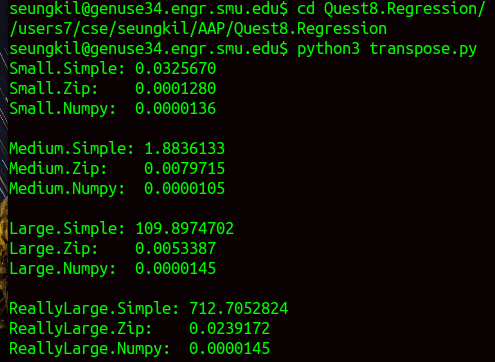
\includegraphics{genuse_quest8.png}
\caption{genuse}
\end{figure}


    % Add a bibliography block to the postdoc
    
    
    
    \end{document}
